
\chapter{Phenomenological and numerical analysis}\label{chap:numerics}
We saw that factorization holds also at NLO .... bla bla\\
It is now interesting to numerically explore our analytical formulae to see if and how the NLO corrections affect the theoretical prediction of the spin asymmetry $A_{UT}^{\sin\phi_S}$. 

We stress the fact that the quantitative analysis of the $A_{UT}^{\sin\phi_S}$ SSA is quite a recent development in the field of QCD hadron structure and phenomenology. In fact, measurements of the $A_{UT}^{\sin\phi_S}$ asymmetry in SIDIS have become available from the HERMES collaboration only in 2020 \cite{hermescollaboration2020azimuthalsingledoublespinasymmetries}. With this set of recent data, the Jefferson Lab Angular Momentum (JAM) collaboration managed to obtain the first ever information about the quark-gluon-quark fragmentation function $\tilde{H}(z) $ within a global QCD analysis \cite{Gamberg2022Htilde}. In the same work, transversity has been extracted including lattice QCD data and proper constraints regarding the Soffer bound, giving the smallest uncertainty on the function so far. With these ingredients, we are now in a position to perform some order of magnitude exploratory estimates of the NLO corrections we calculated. We anticipate the fact that our curves cannot be interpreted as real theoretical predictions, since the twist-3 fragmentation functions $\Im\hat{H}_{FU}^{qg}(z,\zeta)$ and $\Im\hat{H}_{FU}^{\bar{q}q}(z,\zeta)$ are essentially unknown (besides symmetry and few other constraints).

\section{Transversity and the $\tilde{H}$ fragmentation function}
Before dealing with the NLO corrections to the asymmetry, it is useful to visualize the most recent exctractions for both the transversity PDF $h_1^q(x)$ and the quark-gluon-quark fragmentation function $\tilde{H}^q(z)$.  As shown in Fig.~\ref{fig:h1Ht}, transversity is extracted for $u$ and $d$ quarks. Antiquarks distributions can effectively be ignored since they lead to very small contributions and no overall improvement of the quality of the global fit. However, they will play an important role in the analysis of future data from facilities such as the EIC. Here, we set them to zero for simplicity. More interestingly, the $\tilde{H}(z)$ fragmentation function turns out to behave similarly to the first moment of the Collins FF $H_1^{\perp(1)}(z)$. This is not entirely surprising since the two functions are related to each other via an EoMR (Eq.~\eqref{eq:eomr H}) and they are essentially derived from the same underlying quark-gluon-quark correlator \cite{kanazawa_operator_2016}. In \cite{Gamberg2022Htilde}, they extracted favored $\tilde{H}^{\rm fav}$ and unfavored $\tilde{H}^{\rm unf}$ fragmentation functions. These two extractions differ by a sign and describe effects roughly equal in size (with a slightly larger effect for the unfavored channel). By favored hadronization we simply mean the case of a $u$ quark decaying into a positive pion $u\bar{d}$, or a $d$ quark into a negative pion $d\bar{u}$. Explicitly, it is $\tilde{H}^{\rm fav}=\tilde{H}^{u\to \pi^+}=\tilde{H}^{\bar{d}\to \pi^+}=\tilde{H}^{\bar{u}\to \pi^-}=\tilde{H}^{d\to \pi^-}$. Similarly, the unfavored decay channel refers to a "crossing" between the outgoing quark and the detected hadron, i.e. $\tilde{H}^{\rm unf}=\tilde{H}^{u\to \pi^-}=\tilde{H}^{\bar{d}\to \pi^-}=\tilde{H}^{\bar{u}\to \pi^+}=\tilde{H}^{d\to \pi^+}$. Very interestingly, unfavored fragmentation seems to be the dominant effect between the two when it comes to the $A_{UT}^{\sin\phi_S}$ asymmetry, as clearly showcased later. Lastly, we mention that these extractions are performed at the scale $Q^2=4\,\rm{GeV}^2$. For transversity, being a leading twist distribution, a DGLAP scale evolution is implicitly implemented in our numerical analysis through the LHAPDF interface \cite{}. On the other hand, the evolution for $\tilde{H}(z)$ is significantly more involved, as already pointed out in Chap.~\ref{chap:NLO}. The evolution equations are known \cite{Ma_2017} but, unfortunately, there is still no available code that calculates this scale evolution for sub-leading twist fragmentation functions. Ignoring evolution for twist-3 FFs is is not a tremendous problem at LO, but it starts to be a crude approximation when the calculation is pushed at NLO accuracy in $\alpha_S$. This being said, we still believe that an exploratory estimate can be presented, as a proof of principle that NLO corrections to twist-3 distributions play an integral part in the phenomenology of SSAs.


\begin{figure}[h]
    \centering
    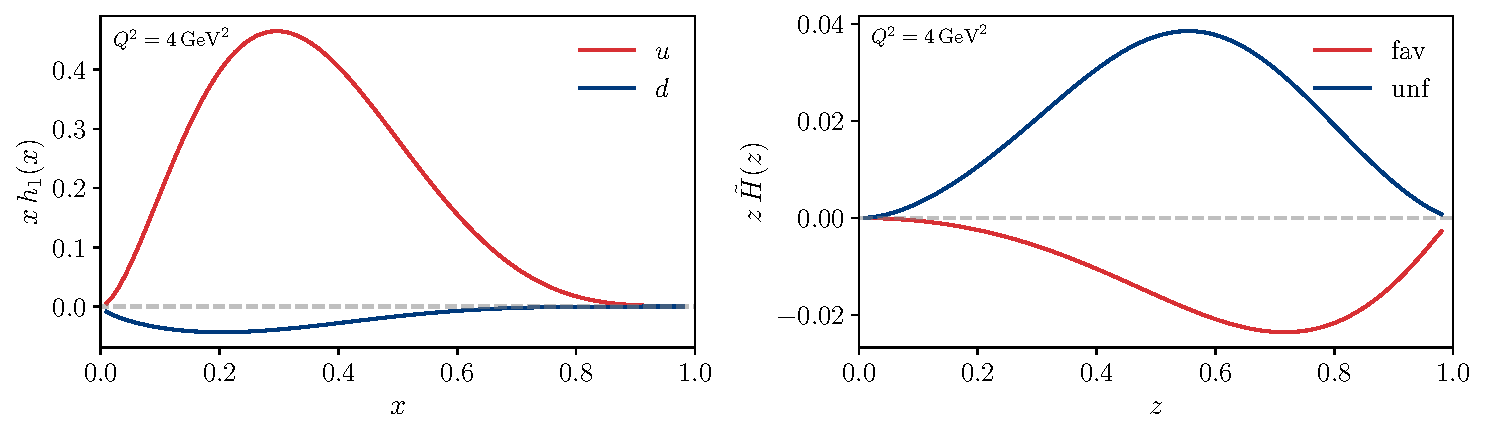
\includegraphics[width=0.99\linewidth]{fig/h1Ht.pdf}
    \caption{Non-perturbative functions entering the numerator of the $A_{UT}^{\sin\phi_S}$ spin asymmetry. Transversity PDF $h_1(x)$ (left) and QGQ fragmentation function $\tilde{H}(z)$ (right). The parametrizations are taken from the JAM22 analysis \cite{Gamberg2022Htilde}.}
    \label{fig:h1Ht}
\end{figure}

\section{The $A_{UT}^{\sin\phi_S}$ spin asymmetry}
In order to compare the $A_{UT}^{\sin\phi_S}$ theoretical prediction against 3D-binned HERMES data we need to point several important aspects. The first being the fact that we are interested in an observable which is integrated over $P_{h\perp}$, the transverse momentum of the detected hadron. As seen in Chap.~\ref{chap:LO}, the only term in the structure function $F_{UT}^{\sin\phi_S}$ that survives the integration over the transverse momentum is the one coupling the transversity PDF $h_1(x)$ and the FF $\tilde{H}(z)$. Hence, in order to be directly sensitive to $\tilde{H}(z)$ in an experiment, one should in principle integrate over all possible transverse hadronic momenta. This however could not be done experimentally at HERMES. For this precise reason, we make the assumption that taking only the $x_B$ and $z_h$ projections of the $A_{UT}^{\sin\phi_S}$ HERMES data is a reasonable approximation \cite{Gamberg2022Htilde}. In practice, we set all the kinematical variables (except the projected one) to their experimental average, easily found in Table 10 Ref.~\cite{hermescollaboration2020azimuthalsingledoublespinasymmetries}. Another important point concerns the (de)polarization factors entering the spin asymmetry. Recalling Chap.~\ref{chap:LO},  the asymmetry can be written as CHECK
\begin{equation}
    A_{UT}^{\sin\phi_S} = \sqrt{2\varepsilon(1+\varepsilon)}\frac{\int d^2P_{h\perp}\,F_{UT}^{\sin\phi_S}(x_B,z_h,P_{h\perp},Q^2)}{\int d^2P_{h\perp}\, F_{UU}(x_B,z_h,P_{h\perp},Q^2)},
\end{equation}
where the $ \sqrt{2\varepsilon(1+\varepsilon)}$ term is the depolarization factor for this polarization case. Conveniently, HERMES asymmetry data is presented both including or excluding this factor. For simplicity, we use the scaled data in which the polarization factor is divided away. Hence, the observable we are going to numerically study is simply given by the ratio of the ($P_{h\perp}$-integrated) structure functions, i.e.
\begin{equation}
    \left(A_{UT}^{\sin\phi_S}\right)_{\rm exp} =\frac{\int d^2P_{h\perp}\,F_{UT}^{\sin\phi_S}(x_B,z_h,P_{h\perp},Q^2)}{\int d^2P_{h\perp}\, F_{UU}(x_B,z_h,P_{h\perp},Q^2)}.
\end{equation}
We stress the fact that the unpolarized structure function at LO is simply given by $F_{UU}=F_{UU,T}$, meaning only transverse photons contribute. However, at NLO more partonic channels become available and therefore the asymmetry denominator becomes $F_{UU}=F_{UU,T}+\varepsilon F_{UU,L}$.

The asymmetry at leading-order in $\alpha_S$ is shown in Fig.~\ref{fig:A_UT_LO}. The leading-order curves are obtained by employing the YYY PDF set REF and ZZZ FF set at LO accuracy, and setting the unprojected kinematical variables to their experimental average, as mentioned before. These curves are analogous to the ones presented in the global analysis in Ref.~\cite{Gamberg2022Htilde}. The fact that the LO projections describe reasonably well HERMES data should not be surprising, since this precise data set has been crucial for the extraction of the $\tilde{H}(z)$ fragmentation function. The HERMES collaboration claims the measurement of the $A_{UT}^{\sin\phi_S}$ asymmetry as one of the most striking results of their analysis. This is because this specific observable has by far the largest twist-3 signal among all sub-leading twist effects. The observation is particularly true for $\pi^-$ production, where the asymmetry is significantly different from zero, of the order of $-2\%$ at least in the studied kinemtical region. Another unexpected and surprising feature revealed by this measurement is the strong kinematic dependence. In fact, the magnitude of the asymmetry significantly rises with increasing $x_B$ and $z_h$, reaching values up to $10\%$ at the edge of the $z_h$ phase space. 
\begin{figure}[h]
    \centering
    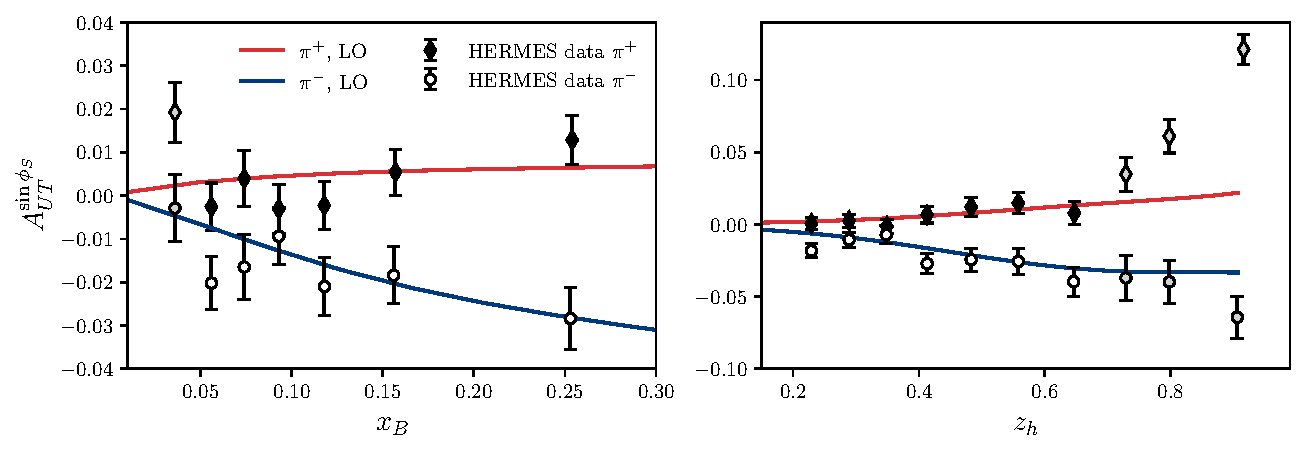
\includegraphics[width=0.99\linewidth]{fig/A_UT_LO.pdf}
    \caption{Projections along $x_B$ and $z_h$ of the (scaled) single spin asymmetry $A_{UT}^{\sin\phi_S}$ at leading-order in $\alpha_S$. As mentioned in \cite{Gamberg2022Htilde}, grey data points in the $x_B$ projection are excluded in the fitting procedure of $\tilde{H}(z)$ since $Q^2\sim 1\,\rm{GeV}^2$ for those data points. Similarly, in the $z_h$ projection the grey data points are not included in other projections and neither are included in the fitting of $\tilde{H}(z)$, since the standard semi-inclusive region corersponds to the kinemtical cut $0.2 <z_h< 0.7$ \cite{hermescollaboration2020azimuthalsingledoublespinasymmetries}.}
    \label{fig:A_UT_LO}
\end{figure}

In order to perform a NLO exploratory study, we need one last ingredient: input fragmentation functions $\Im \hat{H}^{qg}_{FU}(z,\zeta)$ and  $\Im \hat{H}^{\bar{q}q}_{FU}(z,\zeta)$ for all flavors $q$. Since these functions are currently unknown, a real prediction is clearly not possible. We can, though, build some models respecting the currently known constraints and plot the resulting curves for different choices of parameters. A typical parametrization for collinear PDFs and FFs is given by the formula \cite{Gamberg2022Htilde}
\begin{equation}
    P^q(x) \equiv \frac{N^q\, x^{a_q} (1-x)^{b_q}\left( 1+\gamma^q x^{\tilde{a}_q}(1-x)^{\tilde{b}_q}\right)}{\mathbb{B}(a_q+2,b_q+1) + \gamma^q \mathbb{B}(a_q+\tilde{a}_q+2 , b_q + \tilde{b}_q +1)},
\end{equation} 
where $\mathbb{B}(a,b)$ is the Euler beta function. Based on this, we construct some simple models for the fragmentation functions of interest. For simplicity, we set to zero the $\gamma,\tilde{a},\tilde{b}$ parameters, only allowing others to vary. We set
\begin{equation}
    \begin{aligned}
        \Im \hat{H}^{qg}_{FU}(z,\zeta) &= \frac{\tilde{H}(z)}{2 z} \frac{\zeta^{a_q} (1-\zeta)^{b_q}}{\mathbb{B}(1+a_q,b_q)},\\
        \Im \hat{H}^{\bar{q}q}_{FU}(z,\zeta) &= \frac{\tilde{H}(z)}{2 z} \frac{N^q \,\zeta^{c_q} (1-\zeta)^{c_q}}{\mathbb{B}(1+c_q,1+c_q)}.
    \end{aligned}
\end{equation}
It is important to note that in the $qg$ case, our model is guaranteed to satisfy the EoM relation $\tilde{H}(z)/2z=\int\dd\zeta \Im \hat{H}^{qg}_{FU}(z,\zeta)/(1-\zeta)$ by construction. This is the case also for the boundary conditions presented in Chap.~\ref{chap:matrixelements}, such as $\Im \hat{H}^{qg}_{FU}(z,0)=\Im \hat{H}^{qg}_{FU}(z,1)= \partial_\zeta \Im \hat{H}^{qg}_{FU}(z,\zeta)|_{\zeta\to 0}=\partial_\zeta \Im \hat{H}^{qg}_{FU}(z,\zeta)|_{\zeta\to 1}=0$, provided we choose appropriate model parameters. When it comes to the $\bar{q}q$ correlator, it is completely unconstrained. We choose however to model it such that the $z$-dependence precisely matches the quark-gluon-quark FF $\tilde{H}(z)$. After all, these twist-3 objects are all interconnected to one another, and we regard it as a reasonable and very simple assumption. We would expect the $\bar{q}q$ correlator to be symmetric(??) under the exchange of quarks and antiquarks, hence why we set the exponents of $\zeta$ and $(1-\zeta)$ to be equal for a given $q$. 
In order to compare LO and NLO $x$ and $z$ projections, we generate various so called scenarios. We define a scenario as one specific set of model parameters including both fragmentation functions. Meaning, the $k$-th scenario is described by the set $S_k=\{a_u,a_{\bar{u}},a_d,a_{\bar{d}},b_u,b_{\bar{u}},\dots \}$. To generate these scenarios, we sample each parameter from a uniform distribution. EXPLAIN HERE UNIFORM SAMPLING AND LIMITS USED, IF NECESSARY.

The results of our exploratory NLO numerical analysis are presented in Fig.~\ref{fig:A_UT_NLO}. Here, the projections along $x_B$ and $z_h$ of the spin asymmetry are shown, for both $\pi^+$ and $\pi^-$ production. The NLO curves, corresponding to ZZZ different scenarios, exhibit quite different behavior. This is a strong indication of the fact that the NLO corrections to the asymmetry are quite sensitive to the choice of parameters used to describe the QGQ correlators, as well as their model parametrization overall. In principle, one could perform a fit to the experimental data to constrain the QGQ correlators. This is beyond the scope of this work and it may be subject of future investigations.

\begin{figure}[h]
    \centering
    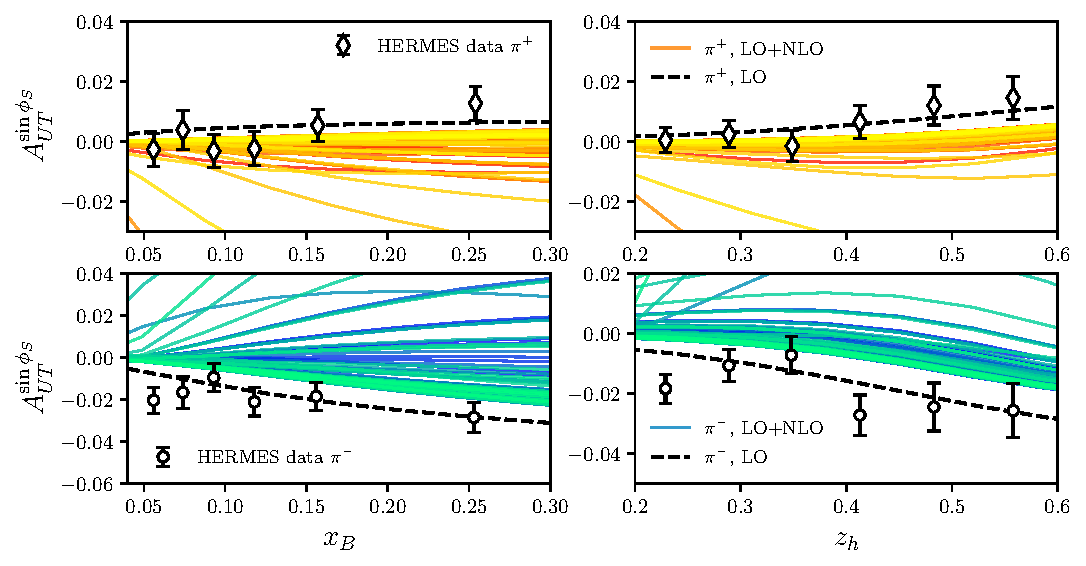
\includegraphics[width=0.99\linewidth]{fig/A_UT_NLO.pdf}
    \caption{Projections along $x_B$ and $z_h$ of the (scaled) single spin asymmetry $A_{UT}^{\sin\phi_S}$. The colored curves correspond to different scenarios $S_j$, i.e. different models for the twist-3 FFs  $\Im \hat{H}^{qg}_{FU}(z,\zeta) $ and $\Im \hat{H}^{\bar{q}q}_{FU}(z,\zeta) $.}
    \label{fig:A_UT_NLO}
\end{figure}

The are essentially two important outcomes of this exploratory NLO study. First, one sees that the NLO corrections to the numerator of the SSA can be large, and not at all negligible. In numerous scenarios we even witness NLO corrections so large that the asymmetry changes sign. This fact alone should be enough to remark the importance of NLO corrections to spin-dependent observables in QCD. We also note the fact that NLO corrections to the numerator of SSAs can be large has been numerically tested in a very similar manner also for single inclusive hadron production $ep\to hX$ \cite{rein2025}. Secondly, the fact that the NLO single-spin asymmetry shows great sensitivity to the set of employed twist-3 matrix elements motivates even more the importance of future precision colliders such as the EIC. In fact, future accurate data collected at larger center-of-mass energies will deepen our understanding of sub-leading twist distribution and fragmentation effects, shedding light on detailed hadron structure and the hadronization mechanism. 














\clearpage